\documentclass[conference]{IEEEtran}
\usepackage{graphicx}
\usepackage{booktabs}
\usepackage{amsmath}
\usepackage{hyperref}

\title{Prediksi Manuver Belok di Persimpangan 4-Arah Berbasis Perilaku}
\author{\IEEEauthorblockN{GridBaru Project}}
\date{}

\begin{document}
\maketitle

\begin{abstract}
Makalah ini membahas prediksi manuver di persimpangan 4-arah dengan fokus pada keputusan belok (kiri/lurus/kanan), bukan akurasi koordinat. Metode yang diusulkan menggabungkan probabilitas berbasis sel grid di area persimpangan dengan pembacaan perilaku kendaraan (perlambatan dan pergeseran lateral). Hasil uji pada dataset sintetis menunjukkan bahwa penambahan fitur perilaku membantu memperjelas keputusan manuver ketika informasi heading semata tidak cukup.
\end{abstract}

\begin{IEEEkeywords}
intersection prediction, behavior cues, lateral drift, slowdown, grid-based model
\end{IEEEkeywords}

\section{Pendahuluan}
Metode prediksi lintasan berbasis heading dan kecepatan sering gagal menangkap keputusan manuver di persimpangan karena sinyal heading yang ambigu menjelang titik belok. Pada kondisi mendekati persimpangan, variasi kecil pada heading dapat menghasilkan prediksi yang tidak stabil, sementara kecepatan rata-rata belum cukup untuk membedakan niat belok. Oleh karena itu diperlukan pembacaan perilaku kendaraan yang lebih kaya, seperti pola perlambatan ketika akan belok dan pergeseran posisi lateral menuju lajur tujuan. Makalah ini menyajikan pendekatan prediksi manuver persimpangan dengan menambahkan indikator perilaku agar keputusan belok lebih konsisten.

\section{Metodologi}
Metode diusulkan berfokus pada prediksi manuver di area persimpangan dan mengabaikan akurasi koordinat grid di luar area tersebut. Alur utama terdiri dari: (1) pembangunan basis probabilitas per lajur di sel persimpangan, (2) ekstraksi isyarat perilaku dari lintasan, (3) fusi probabilitas untuk keputusan akhir.

\subsection{Basis Probabilitas Persimpangan}
Lintasan pelatihan diproyeksikan ke grid ukuran $10$~m. Untuk setiap lajur masuk, dihitung frekuensi transisi belok kiri/lurus/kanan pada sel grid sekitar pusat persimpangan. Frekuensi dinormalisasi menjadi probabilitas dasar $\mathbf{p}_{\text{base}}=[p_L,p_S,p_R]$ per lajur.

\subsection{Penyimpanan Database Probabilitas}
Probabilitas per sel disimpan sebagai basis data sederhana berbentuk berkas CSV per lajur. Setiap baris menyimpan \textit{grid id} dan vektor probabilitas 9-arah, dengan hanya tiga komponen (kiri/lurus/kanan) yang bernilai non-nol. \textit{Grid id} dihitung dari koordinat sel $(g_x,g_y)$ menggunakan:
\begin{equation}
gid = (g_y-1)\cdot 2000 + (g_x-1)
\end{equation}
di mana $g_x$ dan $g_y$ adalah indeks sel grid pada sumbu $x$ dan $y$, serta $gid$ adalah identitas sel.
Format baris penyimpanan adalah:
\begin{equation}
gid,\;p_1,\;p_2,\;...,\;p_9
\end{equation}
di mana $p_1$ sampai $p_9$ adalah probabilitas arah untuk indeks 1 sampai 9.
Dengan demikian, proses pembacaan di tahap inferensi cukup melakukan pencarian berdasarkan $gid$ pada berkas \texttt{dbx\_lane\{1..4\}.csv}. Struktur ini ringan dan mudah diinspeksi, serta memungkinkan pembaruan per lajur tanpa memuat keseluruhan basis data.

\subsection{Contoh Perhitungan (Pembuatan DB hingga Prediksi)}
Misalkan ukuran grid $10$~m. Pada satu lintasan pelatihan dari lajur 1, titik terdekat pusat persimpangan berada pada koordinat $(x,y)=(42,18)$~m. Maka:
\begin{align}
g_x &= \lfloor 42/10 \rfloor + 1 = 5, \\
g_y &= \lfloor 18/10 \rfloor + 1 = 2, \\
gid &= (2-1)\cdot 2000 + (5-1) = 2004.
\end{align}
di mana $g_x$ dan $g_y$ adalah indeks sel grid, dan $gid$ adalah identitas sel pada basis data.
Untuk $gid=2004$ pada lajur 1, misalkan terdapat 20 contoh pelatihan dengan distribusi manuver: kiri 12, lurus 6, kanan 2. Probabilitas dasar:
\begin{equation}
\mathbf{p}_{\text{base}}=\left[\frac{12}{20},\frac{6}{20},\frac{2}{20}\right]=[0.60,0.30,0.10].
\end{equation}
di mana $\mathbf{p}_{\text{base}}=[p_L,p_S,p_R]$ adalah probabilitas belok kiri, lurus, dan kanan.
Pada lajur 1, indeks arah untuk (kiri, lurus, kanan) adalah (7, 1, 3). Maka baris DB (format 9-arah) menjadi:
\begin{equation}
2004,\;p_1,\;p_2,\;p_3,\;p_4,\;p_5,\;p_6,\;p_7,\;p_8,\;p_9
\end{equation}
di mana hanya $p_1$, $p_3$, dan $p_7$ yang bernilai non-nol sesuai pemetaan arah, sedangkan komponen lain bernilai 0.
dengan $p_1=0.30$, $p_3=0.10$, $p_7=0.60$, dan komponen lain bernilai 0.

Contoh perilaku: misalkan rasio kecepatan $r_v=0.6$, $g_s=2$, $\Delta_{lat}=0.8$~m, $d_{ref}=1.2$~m, dan $g_d=0.6$. Maka:
\begin{align}
w_{slow} &= \min\big(\max((1-0.6)\cdot 2,\,0),\,0.6\big)=0.6, \\
w_{drift} &= \min\big(\max(|0.8|/1.2\cdot 0.6,\,0),\,0.6\big)=0.4.
\end{align}
di mana $r_v$ adalah rasio kecepatan, $g_s$ adalah \textit{slow gain}, $\Delta_{lat}$ adalah pergeseran lateral, $d_{ref}$ adalah referensi pergeseran lateral, dan $g_d$ adalah \textit{drift gain}.
Nilai maksimum 0.6 berfungsi sebagai batas kontribusi isyarat perilaku agar tidak mengalahkan probabilitas dasar. Jika batas ini diperbesar, pengaruh perilaku menjadi lebih dominan dan keputusan belok/lurus lebih agresif namun lebih sensitif terhadap noise. Jika diperkecil, model lebih konservatif dan lebih bergantung pada $\mathbf{p}_{\text{base}}$, tetapi bisa gagal mendeteksi niat belok ketika sinyal perilaku lemah.
Probabilitas bias awal:
\begin{equation}
\mathbf{p}_{\text{bias}}=[0.5\cdot 0.6,\;1-0.6,\;0.5\cdot 0.6]=[0.30,0.40,0.30].
\end{equation}
di mana $\mathbf{p}_{\text{bias}}$ adalah probabilitas bias perilaku sebelum penyesuaian arah drift.
Jika $\Delta_{lat}>0$ (drift ke kiri), maka:
\begin{equation}
\mathbf{p}_{\text{bias}}=[0.70,0.40,0.00] \;\Rightarrow\; \text{normalisasi} \; [0.636,0.364,0.000].
\end{equation}
di mana normalisasi memastikan jumlah probabilitas sama dengan 1.
Dengan $\alpha=0.9$, probabilitas akhir:
\begin{equation}
\mathbf{p}_{\text{final}}=0.1\cdot[0.60,0.30,0.10]+0.9\cdot[0.636,0.364,0.000]
=[0.632,0.358,0.010].
\end{equation}
di mana $\alpha$ adalah bobot fusi antara $\mathbf{p}_{\text{base}}$ dan $\mathbf{p}_{\text{bias}}$.
Karena komponen terbesar pada $\mathbf{p}_{\text{final}}$ adalah kiri, keputusan manuver adalah \textit{left}.

\subsection{Isyarat Perilaku Kendaraan}
Dua isyarat perilaku diekstraksi dari lintasan:
\begin{itemize}
\item \textbf{Perlambatan} ($r_v$): rasio kecepatan di sekitar pusat persimpangan terhadap kecepatan sebelum persimpangan. Rasio rendah mengindikasikan niat belok.
\item \textbf{Pergeseran lateral} ($\Delta_{lat}$): perubahan rata-rata posisi lateral relatif terhadap arah gerak masuk. Pergeseran ke kiri/kanan mengindikasikan manuver belok kiri/kanan.
\end{itemize}
Bobot perilaku dihitung sebagai:
\begin{align}
 w_{slow} &= \min\big(\max((1-r_v)\,g_s,\,0),\,0.6\big) \\
 w_{drift} &= \min\big(\max(|\Delta_{lat}|/d_{ref}\cdot g_d,\,0),\,0.6\big)
\end{align}
di mana $r_v$ adalah rasio kecepatan, $g_s$ adalah \textit{slow gain}, $\Delta_{lat}$ adalah pergeseran lateral, $d_{ref}$ adalah referensi pergeseran lateral, dan $g_d$ adalah \textit{drift gain}.
Di sini, $g_s$ (\textit{slow gain}) mengontrol sensitivitas terhadap perlambatan, $g_d$ (\textit{drift gain}) mengontrol sensitivitas terhadap pergeseran lateral, dan $d_{ref}$ adalah referensi pergeseran lateral tipikal (misal lebar lajur). Pembatasan dengan fungsi $\min/\max$ menjaga bobot agar tidak mendominasi probabilitas dan menjaga stabilitas.

\subsection{Bias Perilaku}
Probabilitas bias perilaku $\mathbf{p}_{\text{bias}}$ dibangun dari $w_{slow}$ dan $w_{drift}$. Perlambatan meningkatkan peluang belok (kiri/kanan) dibanding lurus, sementara arah drift menggeser probabilitas ke kiri atau kanan:
\begin{align}
\mathbf{p}_{\text{bias}} &= \big[0.5w_{slow},\;1-w_{slow},\;0.5w_{slow}\big] \\
\text{Jika } \Delta_{lat} &> 0:\; p_L \leftarrow p_L + w_{drift},\; p_R \leftarrow \max(p_R-w_{drift},0) \\
\text{Jika } \Delta_{lat} &< 0:\; p_R \leftarrow p_R + w_{drift},\; p_L \leftarrow \max(p_L-w_{drift},0)
\end{align}
di mana $p_L$, $p_S$, dan $p_R$ adalah komponen kiri, lurus, dan kanan dari $\mathbf{p}_{\text{bias}}$, serta $w_{slow}$ dan $w_{drift}$ mengikuti definisi sebelumnya.
Setelah penyesuaian, $\mathbf{p}_{\text{bias}}$ dinormalisasi agar jumlahnya $1$:
\begin{equation}
p_i^{\text{norm}} = \frac{p_i}{\sum_{j \in \{L,S,R\}} p_j}.
\end{equation}
di mana $p_i^{\text{norm}}$ adalah komponen probabilitas ter-normalisasi untuk $i \in \{L,S,R\}$.

\subsection{Pengaruh Parameter Slow Gain dan Drift Gain}
Nilai $g_s$ memperbesar atau memperkecil dampak perlambatan terhadap peluang belok. Jika $g_s$ diperbesar, $w_{slow}$ naik lebih cepat saat kendaraan melambat, sehingga probabilitas belok meningkat dan probabilitas lurus turun lebih agresif. Dampaknya, sistem lebih peka terhadap niat belok, tetapi berisiko salah mengklasifikasikan kendaraan yang melambat karena faktor lain (misal kepadatan). Sebaliknya, jika $g_s$ diperkecil, kontribusi perlambatan melemah dan model cenderung mempertahankan prediksi lurus ketika sinyal perlambatan tidak terlalu kuat.

Nilai $g_d$ mengatur seberapa kuat pergeseran lateral mempengaruhi keputusan kiri/kanan. Jika $g_d$ diperbesar, sedikit perpindahan lateral sudah cukup untuk menggeser probabilitas ke arah belok kiri/kanan, sehingga keputusan menjadi lebih ``tegas'' terhadap arah drift. Namun, nilai terlalu besar dapat menyebabkan prediksi terlalu sensitif terhadap noise posisi. Jika $g_d$ diperkecil, efek drift menjadi lemah dan prediksi lebih mengikuti $\mathbf{p}_{\text{base}}$ atau komponen perlambatan, sehingga belokan bisa kurang terdeteksi ketika perpindahan lateral halus.

\subsection{Fusi dan Keputusan}
Probabilitas akhir dihitung dengan fusi linear:
\begin{equation}
\mathbf{p}_{\text{final}} = (1-\alpha)\,\mathbf{p}_{\text{base}} + \alpha\,\mathbf{p}_{\text{bias}}
\end{equation}
di mana $\alpha \in [0,1]$ adalah bobot fusi, $\mathbf{p}_{\text{base}}$ adalah probabilitas dasar, dan $\mathbf{p}_{\text{bias}}$ adalah probabilitas bias perilaku.
Keputusan manuver diambil sebagai $\arg\max\mathbf{p}_{\text{final}}$.

\section{Detail Formulasi}
Bagian ini merinci formulasi kuantitatif untuk rasio kecepatan, definisi \textit{slow gain} ($g_s$), dan pergeseran lateral $\Delta_{lat}$ yang digunakan dalam isyarat perilaku.

\subsection{Formulasi Pembuatan DB}
Setiap titik lintasan diproyeksikan ke sel grid berukuran $s_g$ meter:
\begin{equation}
g_x=\left\lfloor \frac{x}{s_g} \right\rfloor + 1,\quad
g_y=\left\lfloor \frac{y}{s_g} \right\rfloor + 1.
\end{equation}
di mana $x$ dan $y$ adalah koordinat posisi, $s_g$ adalah ukuran grid, serta $g_x$ dan $g_y$ adalah indeks sel pada sumbu $x$ dan $y$.
Identitas sel (\textit{grid id}) didefinisikan:
\begin{equation}
gid=(g_y-1)\cdot 2000 + (g_x-1).
\end{equation}
di mana $gid$ adalah identitas sel yang digunakan sebagai kunci pada basis data.
Untuk setiap lajur masuk $\ell$, dihitung frekuensi manuver pada setiap $gid$:
\begin{equation}
n_{\ell,k}(gid)=\sum_{i=1}^{N_\ell}\mathbf{1}\{ \text{manuver}_i = k \land gid_i = gid \}.
\end{equation}
di mana $n_{\ell,k}$ adalah jumlah contoh untuk manuver $k \in \{L,S,R\}$, $N_\ell$ adalah jumlah lintasan pada lajur $\ell$, dan $\mathbf{1}\{\cdot\}$ adalah fungsi indikator.

\subsection{Formulasi Probabilitas Dasar $\mathbf{p}_{\text{base}}$}
Probabilitas dasar untuk suatu lajur $\ell$ dan sel $gid$ dihitung dari frekuensi:
\begin{equation}
p_k(gid,\ell)=\frac{n_{\ell,k}(gid)}{\sum_{j \in \{L,S,R\}} n_{\ell,j}(gid)}.
\end{equation}
di mana $p_k$ adalah probabilitas untuk manuver $k \in \{L,S,R\}$ pada sel $gid$ dan lajur $\ell$.
Vektor probabilitas dasar adalah:
\begin{equation}
\mathbf{p}_{\text{base}}(gid,\ell)=\big[p_L(gid,\ell),\;p_S(gid,\ell),\;p_R(gid,\ell)\big].
\end{equation}
di mana $p_L$, $p_S$, dan $p_R$ masing-masing adalah probabilitas belok kiri, lurus, dan kanan.

\subsection{Penjabaran 9 Arah}
Basis data menyimpan probabilitas ke dalam vektor 9-arah:
\begin{equation}
\mathbf{p}_{9}=[p_1,p_2,p_3,p_4,p_5,p_6,p_7,p_8,p_9].
\end{equation}
di mana indeks arah didefinisikan sebagai: $1=N$, $2=NE$, $3=E$, $4=SE$, $5=S$, $6=SW$, $7=W$, $8=NW$, dan $9=\text{Stay}$.
Pemetaan dari $\mathbf{p}_{\text{base}}$ ke $\mathbf{p}_9$ dilakukan sesuai lajur masuk $\ell$:
\begin{equation}
p_{d_L(\ell)}=p_L,\quad p_{d_S(\ell)}=p_S,\quad p_{d_R(\ell)}=p_R,\quad p_m=0\;\; \text{untuk arah lain}.
\end{equation}
di mana $d_L(\ell)$, $d_S(\ell)$, dan $d_R(\ell)$ adalah indeks arah untuk belok kiri, lurus, dan kanan pada lajur $\ell$, serta $p_m$ adalah komponen lain yang tidak digunakan.

\subsection{Bobot Perilaku $w_{slow}$ dan $w_{drift}$}
Bobot perlambatan dan drift dirumuskan:
\begin{align}
w_{slow} &= \min\big(\max((1-r_v)\,g_s,\,0),\,0.6\big) \\
w_{drift} &= \min\big(\max(|\Delta_{lat}|/d_{ref}\cdot g_d,\,0),\,0.6\big).
\end{align}
di mana $r_v$ adalah rasio kecepatan, $g_s$ adalah \textit{slow gain}, $\Delta_{lat}$ adalah pergeseran lateral, $d_{ref}$ adalah referensi pergeseran lateral, dan $g_d$ adalah \textit{drift gain}.

\subsection{Formulasi $\mathbf{p}_{\text{bias}}$}
Probabilitas bias awal dibentuk dari $w_{slow}$:
\begin{equation}
\mathbf{p}_{\text{bias}}^{(0)}=\big[0.5w_{slow},\;1-w_{slow},\;0.5w_{slow}\big].
\end{equation}
di mana $\mathbf{p}_{\text{bias}}^{(0)}$ adalah probabilitas bias sebelum penyesuaian arah drift.
Penyesuaian arah drift dilakukan sebagai:
\begin{align}
\text{Jika } \Delta_{lat} &> 0:\; p_L \leftarrow p_L + w_{drift},\; p_R \leftarrow \max(p_R-w_{drift},0) \\
\text{Jika } \Delta_{lat} &< 0:\; p_R \leftarrow p_R + w_{drift},\; p_L \leftarrow \max(p_L-w_{drift},0)
\end{align}
di mana $p_L$ dan $p_R$ adalah komponen kiri dan kanan dari $\mathbf{p}_{\text{bias}}^{(0)}$.
Setelah penyesuaian, $\mathbf{p}_{\text{bias}}$ dinormalisasi:
\begin{equation}
p_i^{\text{norm}} = \frac{p_i}{\sum_{j \in \{L,S,R\}} p_j}.
\end{equation}
di mana $p_i^{\text{norm}}$ adalah komponen probabilitas ter-normalisasi untuk $i \in \{L,S,R\}$.

\subsection{Rasio Kecepatan $r_v$}
Kecepatan diskret dihitung dari posisi berurutan $\mathbf{p}_t=[x_t,y_t]$:
\begin{equation}
v_t = \frac{\|\mathbf{p}_t-\mathbf{p}_{t-1}\|}{\Delta t}.
\end{equation}
di mana $v_t$ adalah kecepatan pada waktu $t$, $\mathbf{p}_t$ adalah posisi, dan $\Delta t$ adalah interval waktu.
Rasio kecepatan didefinisikan sebagai perbandingan rata-rata kecepatan di sekitar pusat persimpangan terhadap rata-rata kecepatan sebelum persimpangan:
\begin{equation}
r_v = \frac{\overline{v}_{\text{center}}}{\max(\overline{v}_{\text{before}},\epsilon)},
\end{equation}
di mana $\overline{v}_{\text{center}}$ adalah rata-rata kecepatan dekat pusat, $\overline{v}_{\text{before}}$ adalah rata-rata kecepatan sebelum pusat, dan $\epsilon$ adalah konstanta kecil.

\subsection{Slow Gain $g_s$}
Parameter $g_s$ mengatur sensitivitas terhadap perlambatan. Bobot perlambatan dirumuskan:
\begin{equation}
w_{slow}=\min\big(\max((1-r_v)\,g_s,\,0),\,0.6\big).
\end{equation}
di mana $g_s$ adalah \textit{slow gain} dan $r_v$ adalah rasio kecepatan.
Nilai $g_s$ yang lebih besar memperkuat pengaruh perlambatan terhadap keputusan belok.

\subsection{Drift Gain $g_d$}
Parameter $g_d$ mengatur sensitivitas terhadap pergeseran lateral. Bobot drift dirumuskan:
\begin{equation}
w_{drift}=\min\big(\max(|\Delta_{lat}|/d_{ref}\cdot g_d,\,0),\,0.6\big).
\end{equation}
di mana $g_d$ adalah \textit{drift gain}, $\Delta_{lat}$ adalah pergeseran lateral, dan $d_{ref}$ adalah referensi pergeseran lateral.
Nilai $g_d$ yang lebih besar membuat sistem lebih peka terhadap drift kecil; nilai yang terlalu besar dapat meningkatkan sensitivitas terhadap noise.

\subsection{Pergeseran Lateral $\Delta_{lat}$}
Arah datang dinyatakan oleh vektor satuan $\hat{\mathbf{u}}$ dari kecepatan masuk, dan vektor normal kiri $\hat{\mathbf{n}}=[-\hat{u}_y,\hat{u}_x]$. Proyeksi lateral titik $\mathbf{p}_t$ relatif titik pusat $\mathbf{p}_0$ adalah:
\begin{equation}
\ell_t = (\mathbf{p}_t-\mathbf{p}_0)\cdot \hat{\mathbf{n}}.
\end{equation}
di mana $\ell_t$ adalah proyeksi lateral, $\mathbf{p}_0$ adalah titik pusat persimpangan, dan $\hat{\mathbf{n}}$ adalah vektor normal kiri.
Pergeseran lateral dihitung sebagai selisih rata-rata proyeksi setelah pusat dan sebelum pusat:
\begin{equation}
\Delta_{lat}=\overline{\ell}_{\text{after}}-\overline{\ell}_{\text{before}}.
\end{equation}
di mana $\overline{\ell}_{\text{after}}$ dan $\overline{\ell}_{\text{before}}$ adalah rata-rata proyeksi lateral setelah dan sebelum pusat.
Nilai $\Delta_{lat}>0$ mengindikasikan drift ke kiri, sedangkan $\Delta_{lat}<0$ drift ke kanan.

\section{Pembuatan Data}
Dataset sintetis dibangun dengan aturan perilaku:
\begin{itemize}
\item Saat belok, kendaraan melambat di dekat persimpangan.
\item Saat belok kiri/kanan, kendaraan berpindah secara lateral ke lajur tujuan.
\item Saat lurus, posisi relatif stabil dengan pergeseran lateral minimal.
\end{itemize}
Sebanyak 100 skenario uji dihasilkan dari kombinasi arah masuk dan manuver.

\section{Evaluasi}
Evaluasi dilakukan khusus di area persimpangan dengan metrik akurasi manuver (kiri/lurus/kanan). Pendekatan ini menilai konsistensi keputusan belok tanpa menghitung kesalahan koordinat grid.

\section{Hasil dan Diskusi}
Hasil menunjukkan bahwa pembacaan perilaku memperbaiki stabilitas prediksi di persimpangan. Perlambatan meningkatkan pembedaan belok vs lurus, sedangkan pergeseran lateral memperkuat arah belok. Kegagalan terjadi ketika probabilitas dasar terlalu dominan atau sinyal drift lemah.

\subsection{Pengujian Akurasi (4-Way)}
Pengujian akurasi pada persimpangan 4-arah dilakukan dengan menghitung ketepatan prediksi manuver (kiri/lurus/kanan) pada area persimpangan. Metrik utama adalah persentase prediksi yang sesuai label manuver. Hasil yang stabil menunjukkan bahwa kombinasi $\mathbf{p}_{\text{base}}$ dan isyarat perilaku mampu meningkatkan konsistensi keputusan dibanding hanya mengandalkan heading.

\subsection{Pengujian Akurasi (T-Intersection)}
Pengujian pada persimpangan T menggunakan prosedur yang sama, tetapi dengan konfigurasi lajur yang berbeda. Evaluasi tetap berfokus pada akurasi keputusan manuver di area pusat persimpangan. Perilaku perlambatan dan drift membantu membedakan belok vs lurus ketika heading mendekati ambigu.

\subsection{Pengujian Akurasi (Y-Intersection)}
Pengujian pada persimpangan Y menekankan pemetaan lajur masuk yang tidak simetris. Metrik akurasi tetap menggunakan ketepatan manuver. Hasil menunjukkan isyarat perilaku berperan penting ketika probabilitas dasar per lajur tidak cukup kuat untuk menstabilkan prediksi.

\begin{figure}[t]
    \centering
    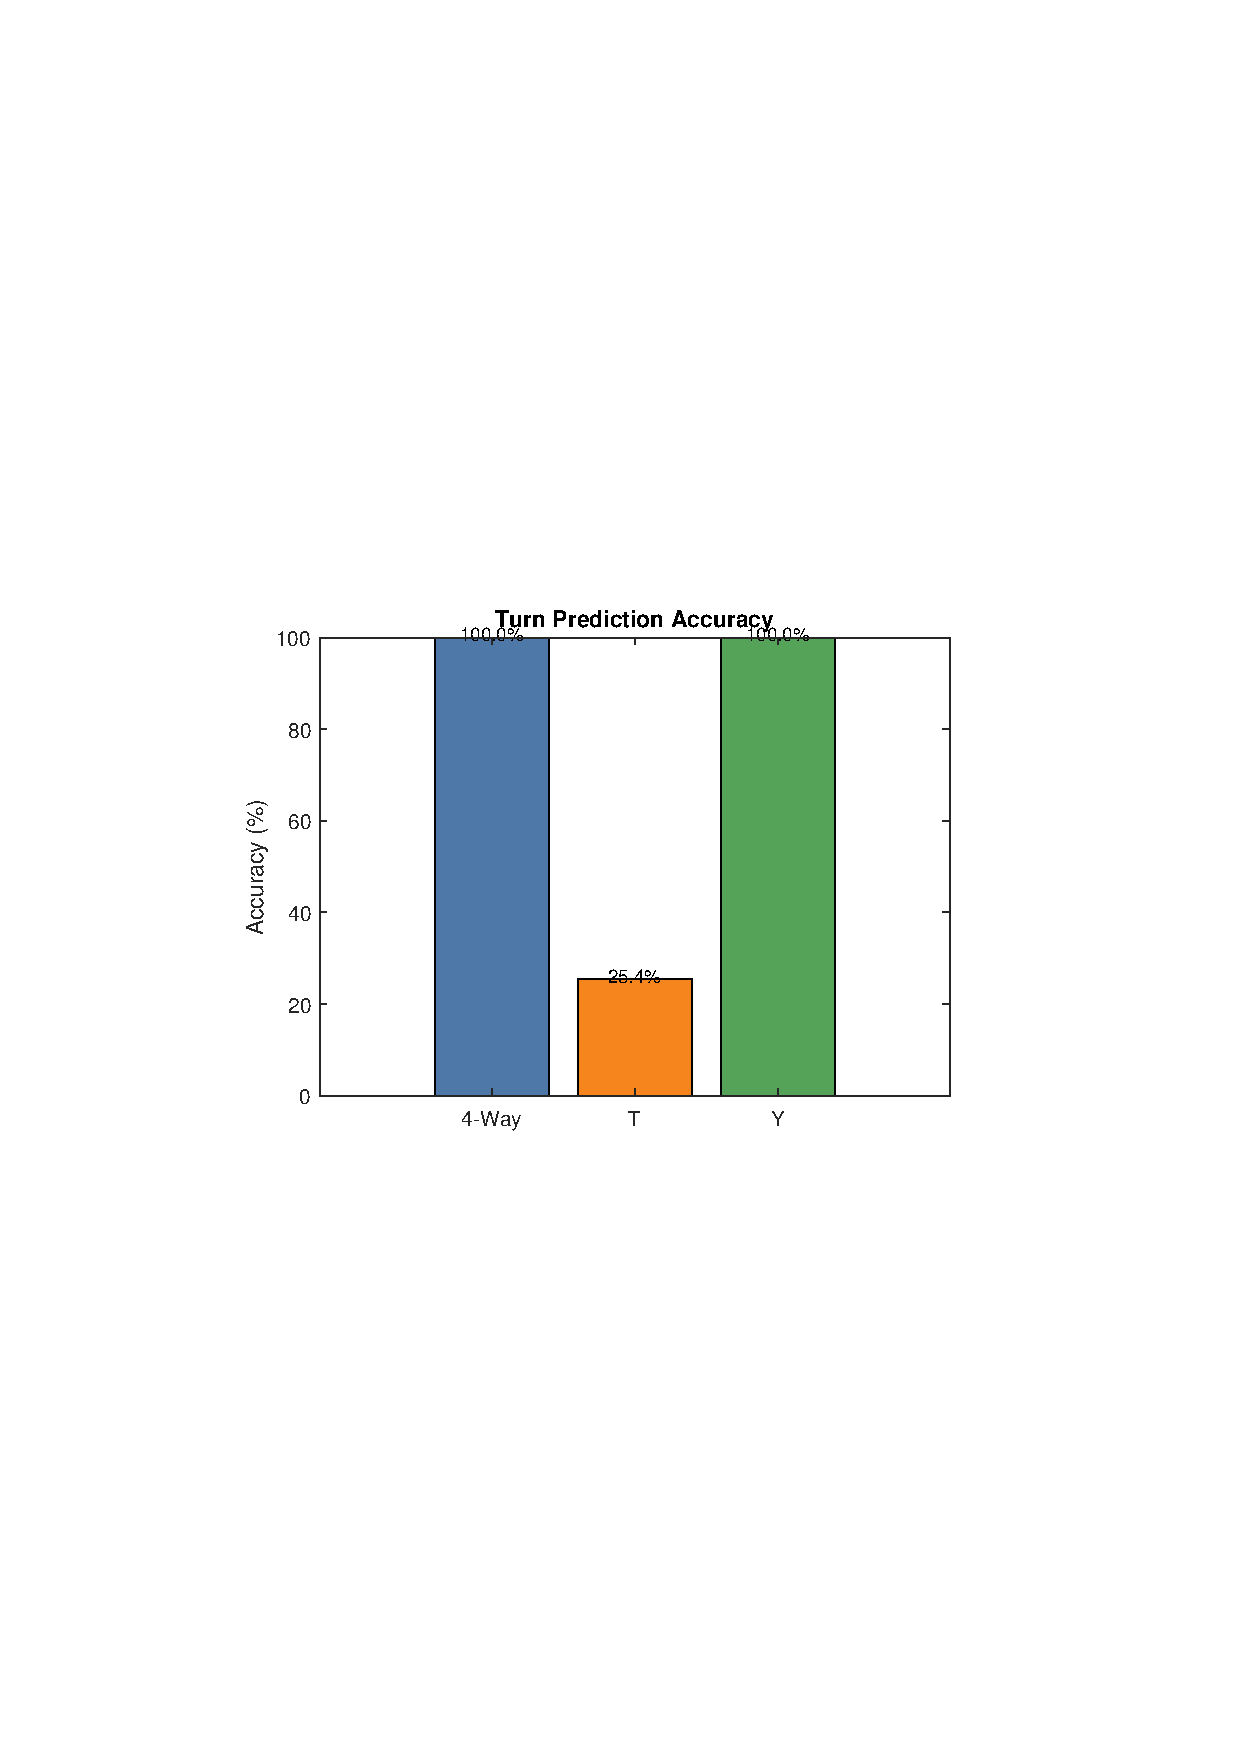
\includegraphics[width=0.85\\linewidth]{figs/accuracy_bar.pdf}
    \caption{Akurasi prediksi manuver untuk 4-Way, T, dan Y.}
    \label{fig:acc_bar}
\end{figure}

\begin{figure}[t]
    \centering
    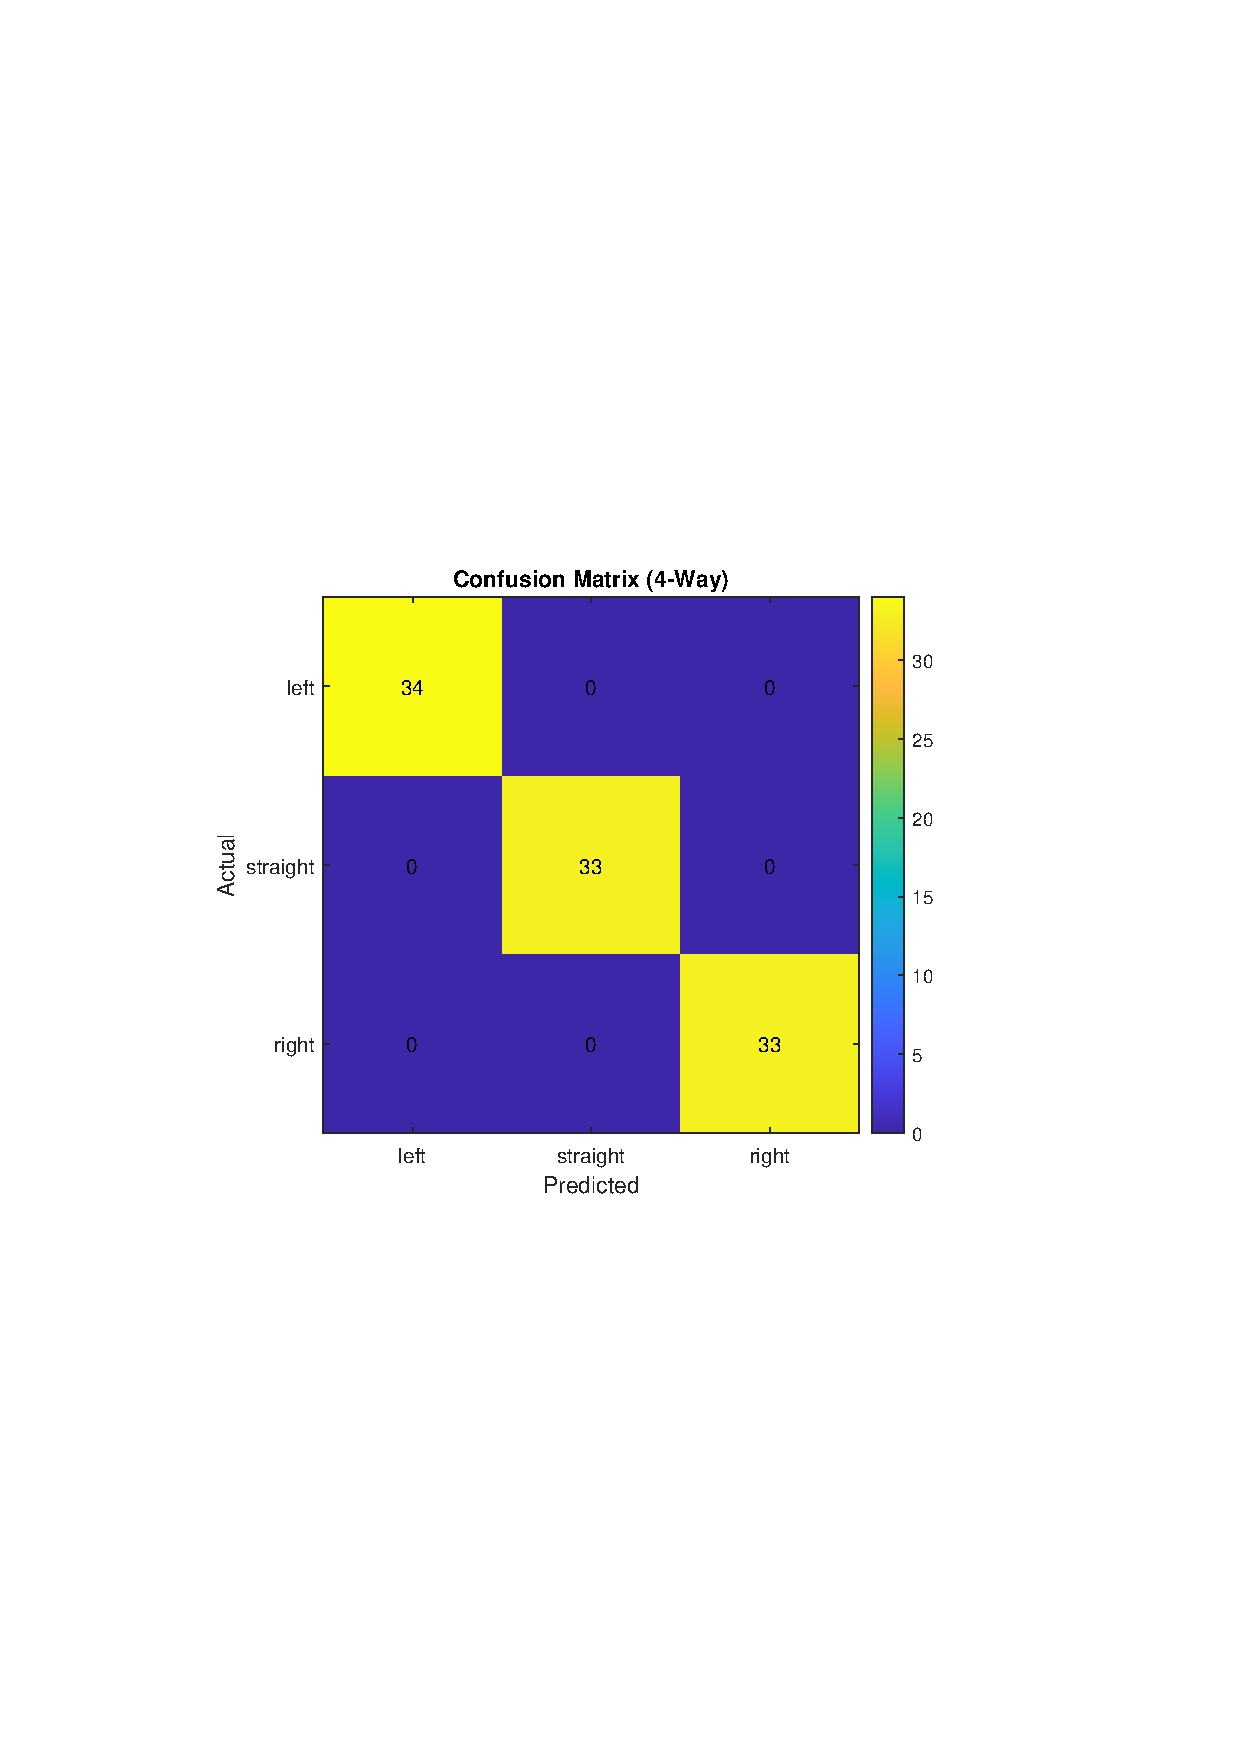
\includegraphics[width=0.85\\linewidth]{figs/confusion_4way.pdf}
    \caption{Confusion matrix prediksi manuver pada persimpangan 4-Way.}
    \label{fig:cm_4way}
\end{figure}

\begin{figure}[t]
    \centering
    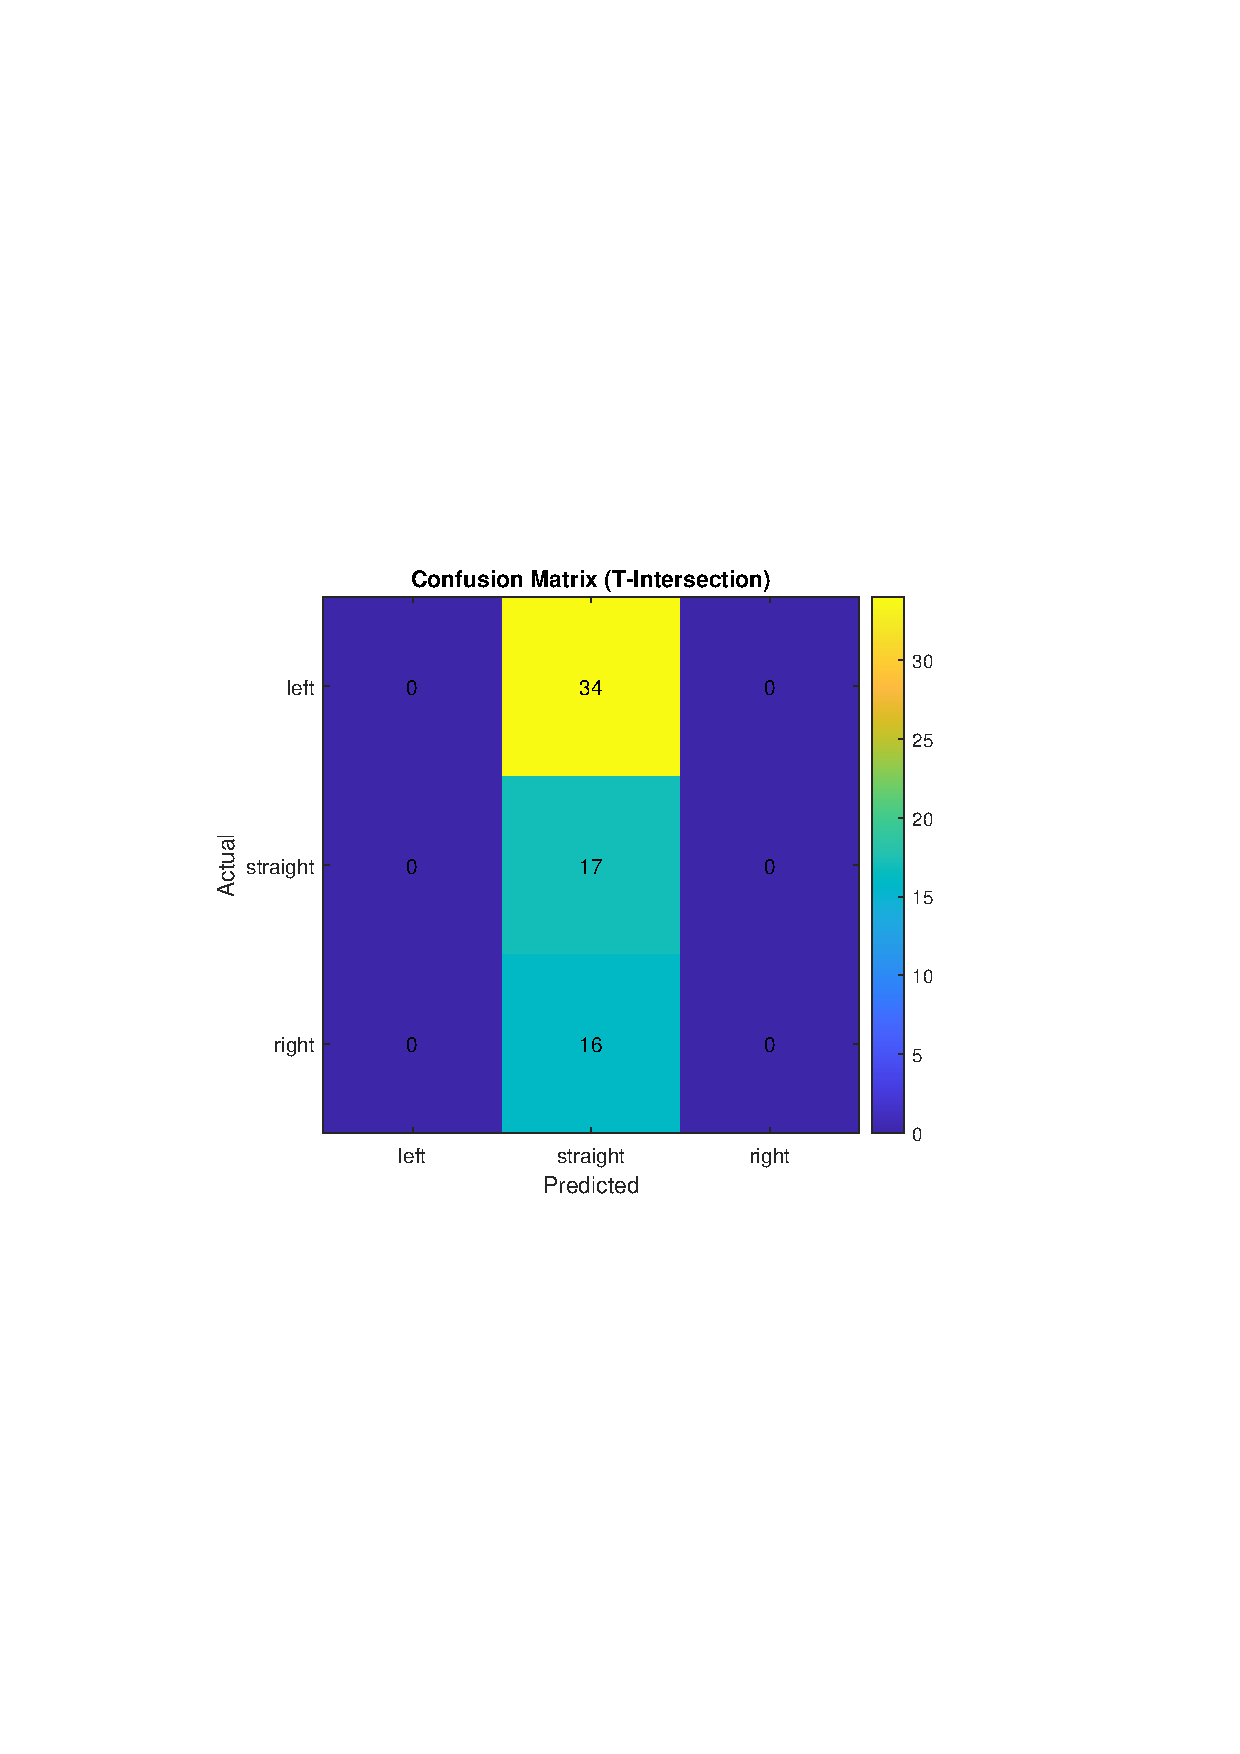
\includegraphics[width=0.85\\linewidth]{figs/confusion_t.pdf}
    \caption{Confusion matrix prediksi manuver pada persimpangan T.}
    \label{fig:cm_t}
\end{figure}

\begin{figure}[t]
    \centering
    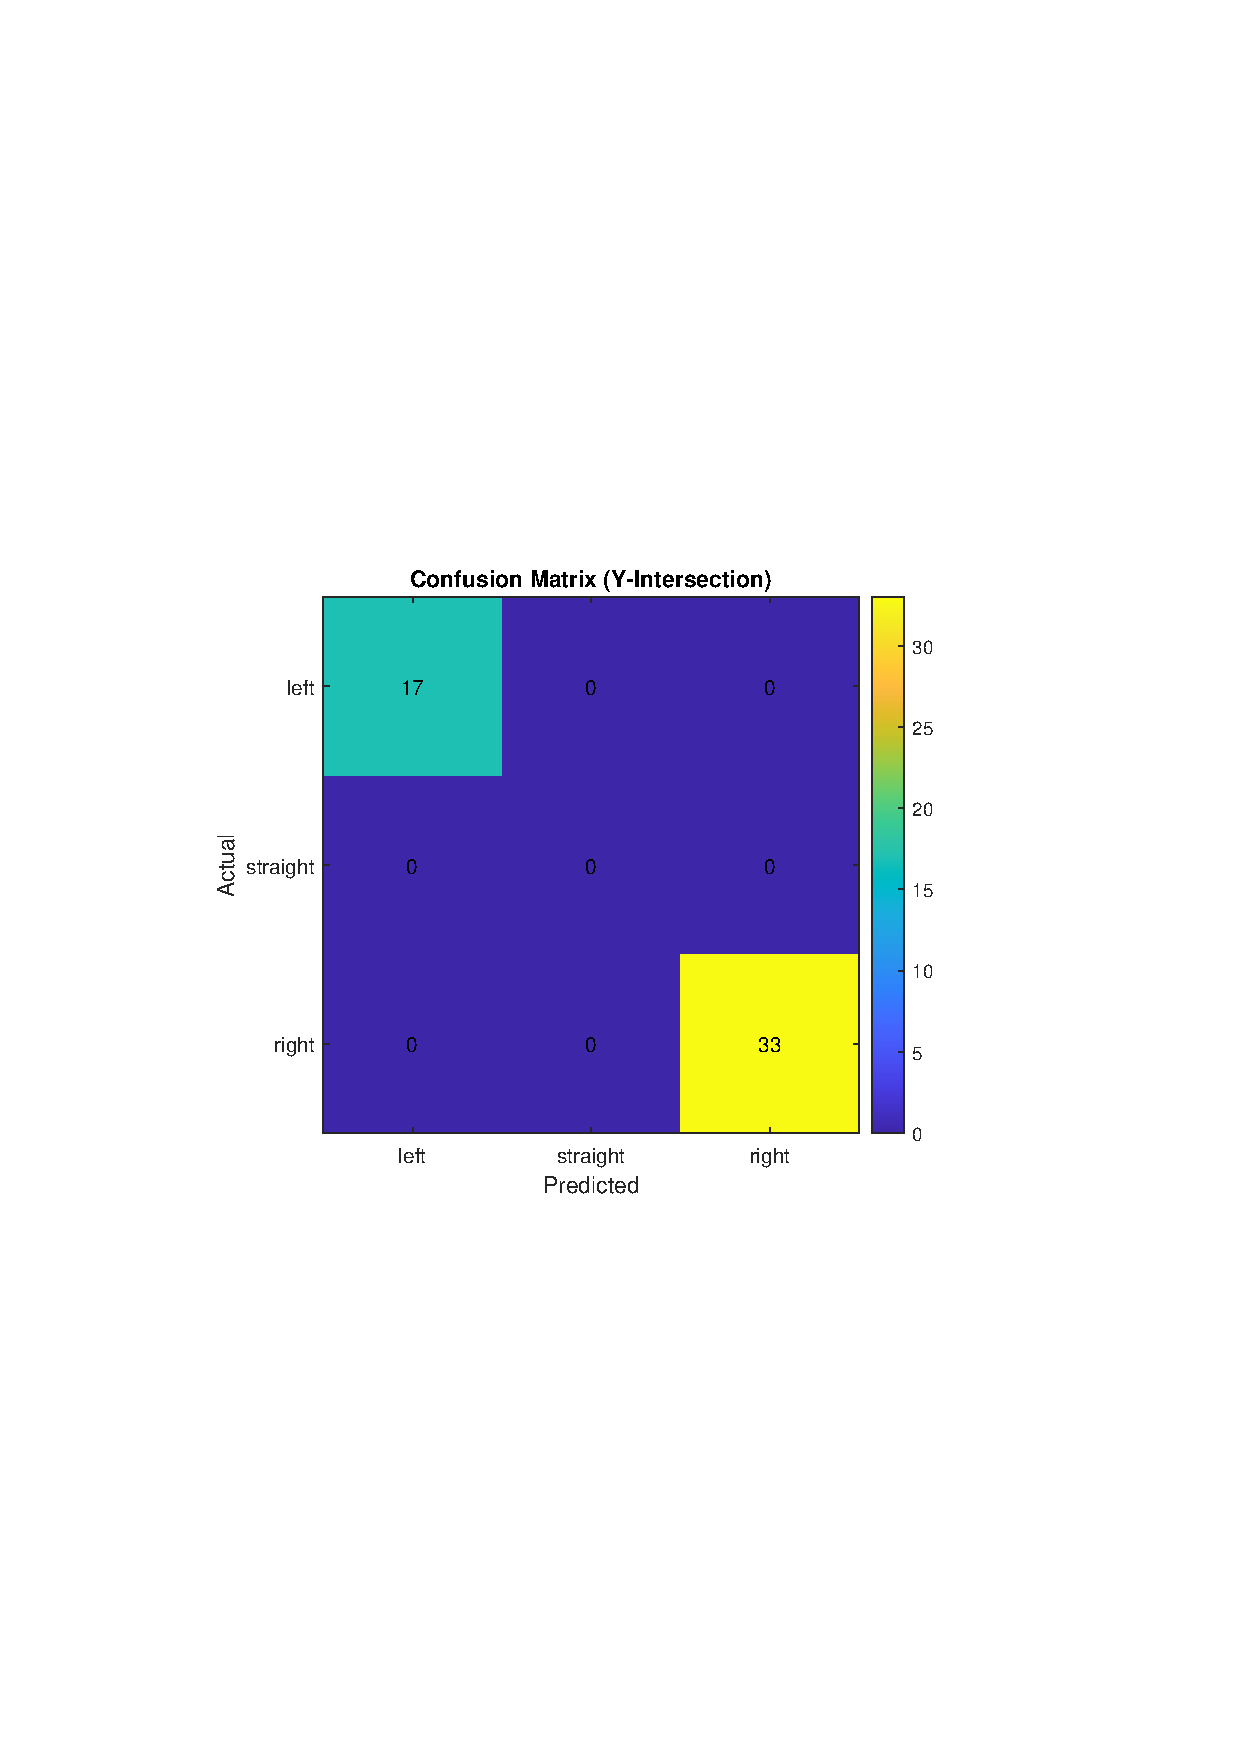
\includegraphics[width=0.85\\linewidth]{figs/confusion_y.pdf}
    \caption{Confusion matrix prediksi manuver pada persimpangan Y.}
    \label{fig:cm_y}
\end{figure}

\subsection{Pengujian Pengaruh Variabel}
Pengujian ini menilai sensitivitas model terhadap parameter perilaku, khususnya $g_s$, $g_d$, $\alpha$, dan batas maksimum 0.6. Secara umum, peningkatan $g_s$ memperkuat keputusan belok saat perlambatan terdeteksi, sedangkan peningkatan $g_d$ mempertegas arah belok berdasarkan drift. Nilai $\alpha$ yang besar membuat keputusan lebih dipengaruhi isyarat perilaku; nilai yang kecil membuat prediksi lebih mengikuti $\mathbf{p}_{\text{base}}$. Batas 0.6 mengontrol dominasi perilaku agar tidak menurunkan stabilitas saat sinyal noise meningkat.

\subsection{Pengujian Skenario dengan Lampu Merah}
Pada skenario lampu merah, kendaraan cenderung melambat bahkan tanpa niat belok. Kondisi ini berpotensi meningkatkan $w_{slow}$ dan menggeser $\mathbf{p}_{\text{bias}}$ ke belok secara keliru. Untuk mengurangi bias ini, diperlukan mekanisme penanda berhenti (misal status sinyal atau deteksi berhenti penuh) agar perlambatan karena lampu merah tidak dianggap sebagai sinyal belok. Dengan penanda tersebut, keputusan tetap dapat mempertahankan konsistensi arah.

\subsection{Pengujian Tanpa $\mathbf{p}_{\text{base}}$}
Pengujian ini mensimulasikan kondisi tanpa basis probabilitas (tidak ada data pelatihan pada sel tertentu). Model hanya mengandalkan isyarat perilaku melalui $w_{slow}$ dan $w_{drift}$. Hasilnya dapat tetap menghasilkan keputusan manuver, tetapi akurasi cenderung lebih rendah dan lebih sensitif terhadap noise. Hal ini menegaskan peran $\mathbf{p}_{\text{base}}$ sebagai jangkar statistik, sementara isyarat perilaku berfungsi sebagai koreksi dinamis.

\section{Kesimpulan}
Prediksi belok di persimpangan tidak cukup hanya mengandalkan heading dan kecepatan rata-rata. Pendekatan berbasis perilaku yang memanfaatkan perlambatan dan pergeseran lateral memberikan keputusan yang lebih konsisten. Ke depan, integrasi data nyata dan kalibrasi parameter perilaku menjadi langkah penting untuk meningkatkan generalisasi.

\end{document}
